% Makros zur Kompatibilitaet mit Onlinemodul: 
 \providecommand{\MoIl}[1][]{\mbox{}#1]\mathopen{}} 
 \providecommand{\MoIr}[1][]{#1[\mbox{}} 
 \providecommand{\MIntvlSep}{;} 
 \providecommand{\MElSetSep}{\, ; \, } 
 \begin{MAufgabe}{Lineare Betrags(un)gleichungen}{vr, 2016, MaTeX}
L\"osen Sie die Gleichung
$$
 \MDS 3\left| 5\, x + 3 \right|-4= 4 \left| -2 \right| 4
$$  

\ifLsg\MLoesung

Im ersten Schritt k\"onnen die Terme au\ss{}erhalb der Betragszeichen zusammengefasst werden:

\begin{align*} 
 3\left| 5\, x + 3 \right|-4= 4 \left| -2 \right| 4\\ 
\Leftrightarrow3\, \left|5\, x + 3\right| - 16= 0 
 \end{align*}

F\"ur diese Gleichung haben wir 2 F\"alle zu unterscheiden: 
\begin{enumerate}
\item $ \MDS 
0 \leq 5\, x + 3
\Leftrightarrow - \frac{3}{5} \leq x\Leftrightarrow x \in [ - \frac{3}{5} \, \MIntvlSep \, \infty\MoIr $ 
\item $ \MDS 
5\, x + 3 < 0
\Leftrightarrow x < - \frac{3}{5}\Leftrightarrow x \in \MoIl  -\infty \, \MIntvlSep \, - \frac{3}{5}\MoIr $ 
\end{enumerate} 
Fallunterscheidung: 

 \begin{enumerate} 
 \item Sei $ \MDS x\in[ - \frac{3}{5} \, \MIntvlSep \, \infty\MoIr $. 
 In diesem Fall gilt:  
  $ \MDS \left| 5\, x + 3\right|=5\, x + 3$. \\ 
 Damit ist die Gleichung 
 $$ 
3\, \left|5\, x + 3\right| - 16= 0
$$
 \"aquivalent zur Gleichung
 $$ 
3\left(5\, x + 3\right)-16= 0 
$$  
$$ 
 \Leftrightarrow 15\, x - 7= 0 
$$  
$$ \Leftrightarrow x = \frac{7}{15} . 
 $$ 
 Die L\"osung muss auch die Fallbedingung $x\in [ - \frac{3}{5} \, \MIntvlSep \, \infty\MoIr  $ erf\"ullen. Die gefundene L\"osung $x=\frac{7}{15}$ erf\"ullt die Fallbedingung  $x\in [ - \frac{3}{5} \, \MIntvlSep \, \infty\MoIr $ und deshalb ist  $$
 \mathcal{L}_{1}=\left\{\frac{7}{15}\right\}
 $$ 
\item Sei $ \MDS x\in\MoIl  -\infty \, \MIntvlSep \, - \frac{3}{5}\MoIr $. 
 In diesem Fall gilt:  
  $ \MDS \left| 5\, x + 3\right|= - 5\, x - 3$. \\ 
 Damit ist die Gleichung 
 $$ 
3\, \left|5\, x + 3\right| - 16= 0
$$
 \"aquivalent zur Gleichung
 $$ 
3\left( - 5\, x - 3\right)-16= 0 
$$  
$$ 
 \Leftrightarrow  - 15\, x - 25= 0 
$$  
$$ \Leftrightarrow x = - \frac{5}{3} . 
 $$ 
 Die L\"osung muss auch die Fallbedingung $x\in \MoIl  -\infty \, \MIntvlSep \, - \frac{3}{5}\MoIr  $ erf\"ullen. Die gefundene L\"osung $x=- \frac{5}{3}$ erf\"ullt die Fallbedingung  $x\in \MoIl  -\infty \, \MIntvlSep \, - \frac{3}{5}\MoIr $ und deshalb ist  $$
 \mathcal{L}_{2}=\left\{- \frac{5}{3}\right\}
 $$ 
 \end{enumerate} 
  Die L\"osungsmenge des Ausgangsproblems ist die Vereinigung der einzelnen L\"osungsmengen: 
$$ \mathcal{L} = \mathcal{L}_{1} \cup \mathcal{L}_{2} 
 = \left\{\frac{7}{15}\right\}\cup \left\{- \frac{5}{3}\right\} 
  = \left\{\frac{7}{15}\MElSetSep- \frac{5}{3}\right\} 
 . $$ 
 
 \begin{center}
 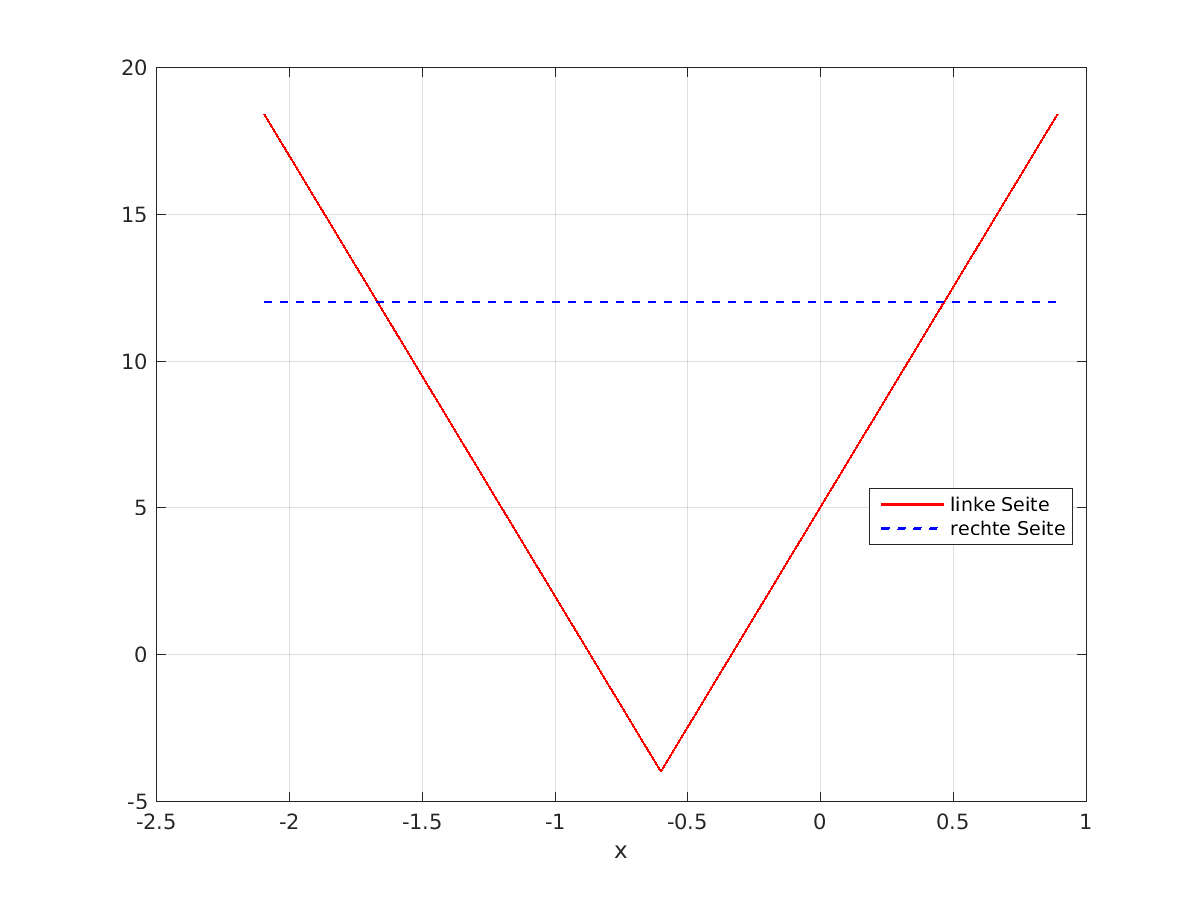
\includegraphics[width=0.8\linewidth]{Abb_zur_Ag_autogenerated_ineq_12.png} \end{center}
 
\else\relax\fi
 \end{MAufgabe}